\documentclass{article}
\usepackage{ee105}

%% Makes figure labels bold
\usepackage[labelfont=bf]{caption}

\begin{document}
\thispagestyle{plain}

\tutorial{HP 6235A DC Power Supply}

\section{Introduction}
The DC power supply is simple, so this tutorial only contains a few bulleted notes and a simple example. There is an image of the front panel interface in Figure \ref{frontpanel}.

\section{Interface Notes}
\begin{itemize}
\item The power suppy can output independent values on the +6V and $\pm$\unit{18}{\volt} outputs, adjusted with separate knobs. All outputs are always ``on,'' though the analog meter can only display one value at a time.
\item For the \unit{18}{\volt} outputs, use the blue numbers on the analog meter. For the \unit{6}{\volt} output, use the black numbers.
\item The Track knob is used to set the \unit{-18}{\volt} output as a proportion of the \unit{+18}{\volt} output setting. If the \unit{+18}{\volt} output is set to \unit{9}{\volt}, then the \unit{-18}{\volt} output will be \unit{-9}{\volt} when the Track knob is turned all the way clockwise. The \unit{-18}{\volt} output can be moved closer to zero (COM ground) by turning the Track knob counterclockwise.
\item The power supply can be switched into a current-source mode by toggling the V/A button on the left side of the METER section. For these labs you will only use the voltage mode, so the button should always be out.
\end{itemize}


\begin{figure}[!htb]
  \centering
  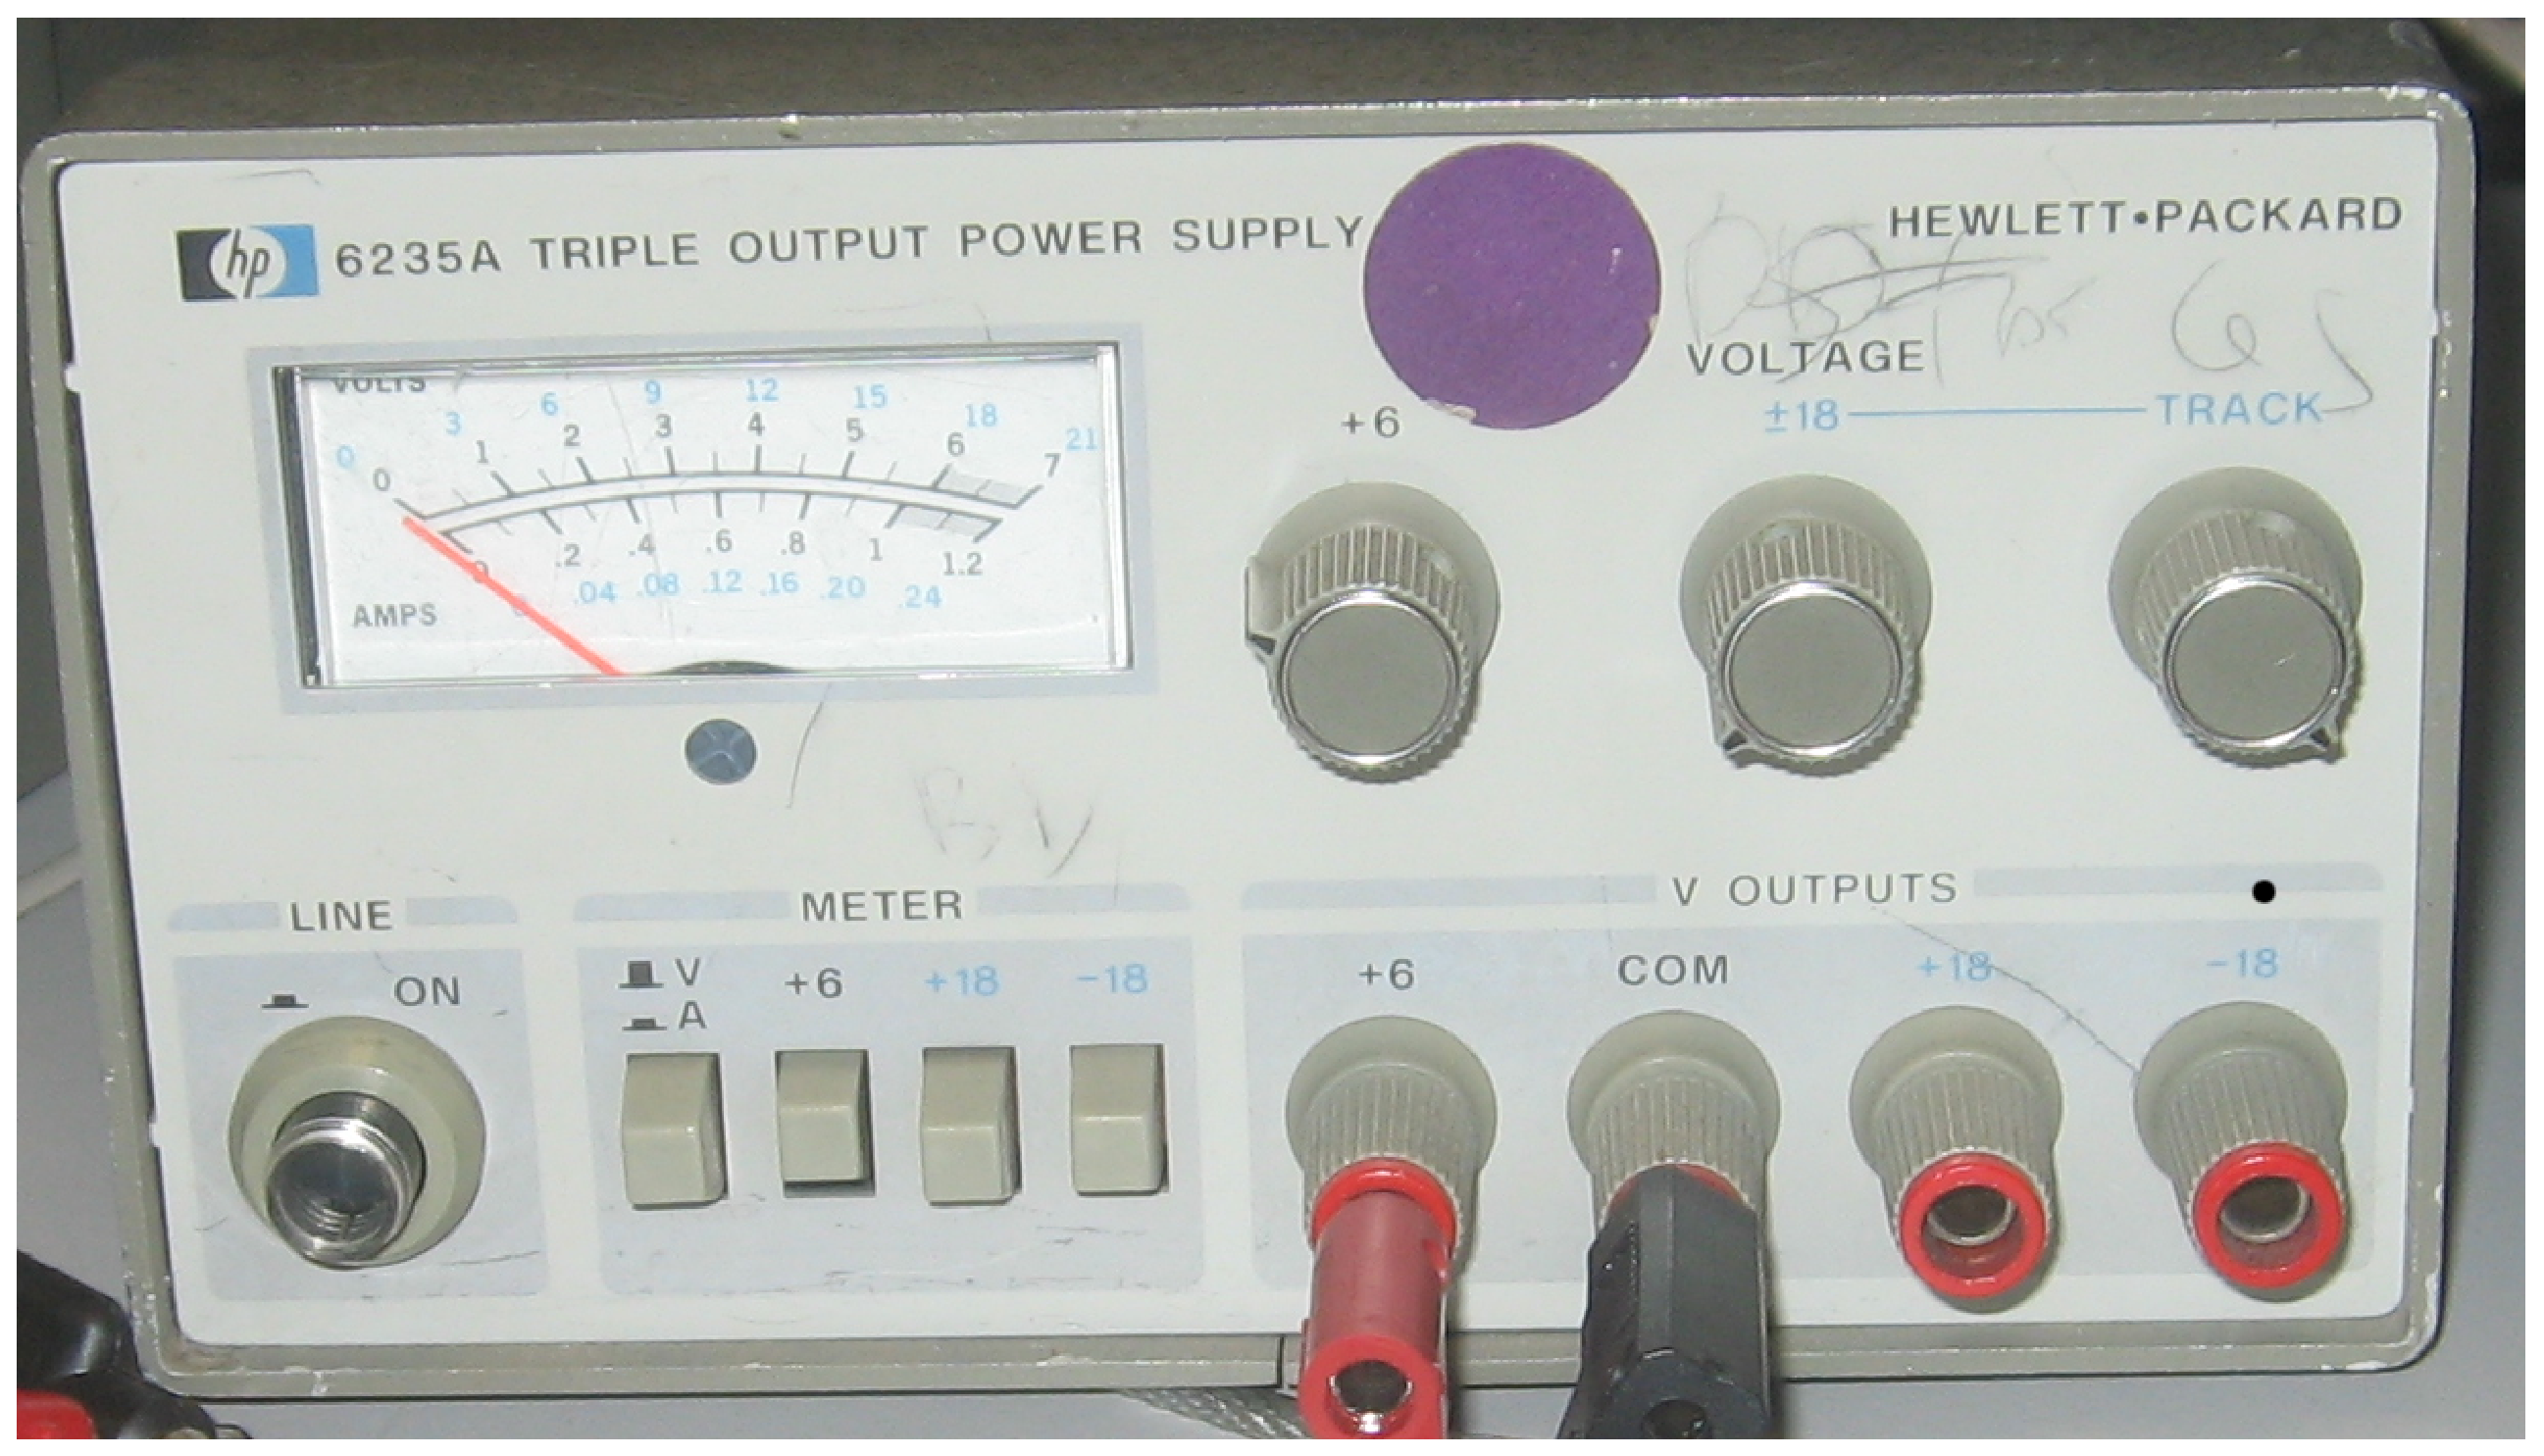
\includegraphics[width=5.0in]{HP6235A.eps}
  \caption{HP6235A front panel.}
  \label{frontpanel}
\end{figure}

\section{Examples}
Here are all of the steps necessary to set up \unit{+9}{\volt} and \unit{-9}{\volt} supply rails.
\begin{enumerate}
\item Turn on the power supply with the lower-left power button.
\item Check to be sure the V/A button in the METER section is out.
\item Press the \unit{+18}{\volt} button in the METER section to view the voltage setting for that output. Move the $\pm$\unit{18}{\volt} knob until the needle points to the blue 9 marking at the top of the meter.
\item Press the \unit{-18}{\volt} button in the METER section to view the voltage setting for that output. Adjust the Track knob all the way clockwise, and verify that the needle points to the blue 9 marking at the top of the meter.
\item Connect cables to the \unit{+18}{\volt} and \unit{-18}{\volt} output ports, which will be \unit{+9}{\volt} and \unit{-9}{\volt}, respectively. 
\item \textbf{The power supply has a floating ground}, so you can cascade them in series to reach higher voltages. Other equipment is earth-grounded.
\end{enumerate}

\end{document} 
